\documentclass{standalone}

\usepackage[latin1]{inputenc}
\usepackage{amsmath}
\usepackage{amssymb}
\usepackage{amsthm}

\usepackage{tikz}
\usetikzlibrary{arrows,calc}

%% generates a tightly fitting border around the work
%\usepackage[active,tightpage]{preview}
%\PreviewEnvironment{tikzpicture}
%\setlength\PreviewBorder{0.5mm}
%%\renewcommand\PreviewBbAdjust{-\PreviewBorder 1mm -1.15mm -0.85mm}

\usepackage{color}

%\pagestyle{empty}

\begin{document}

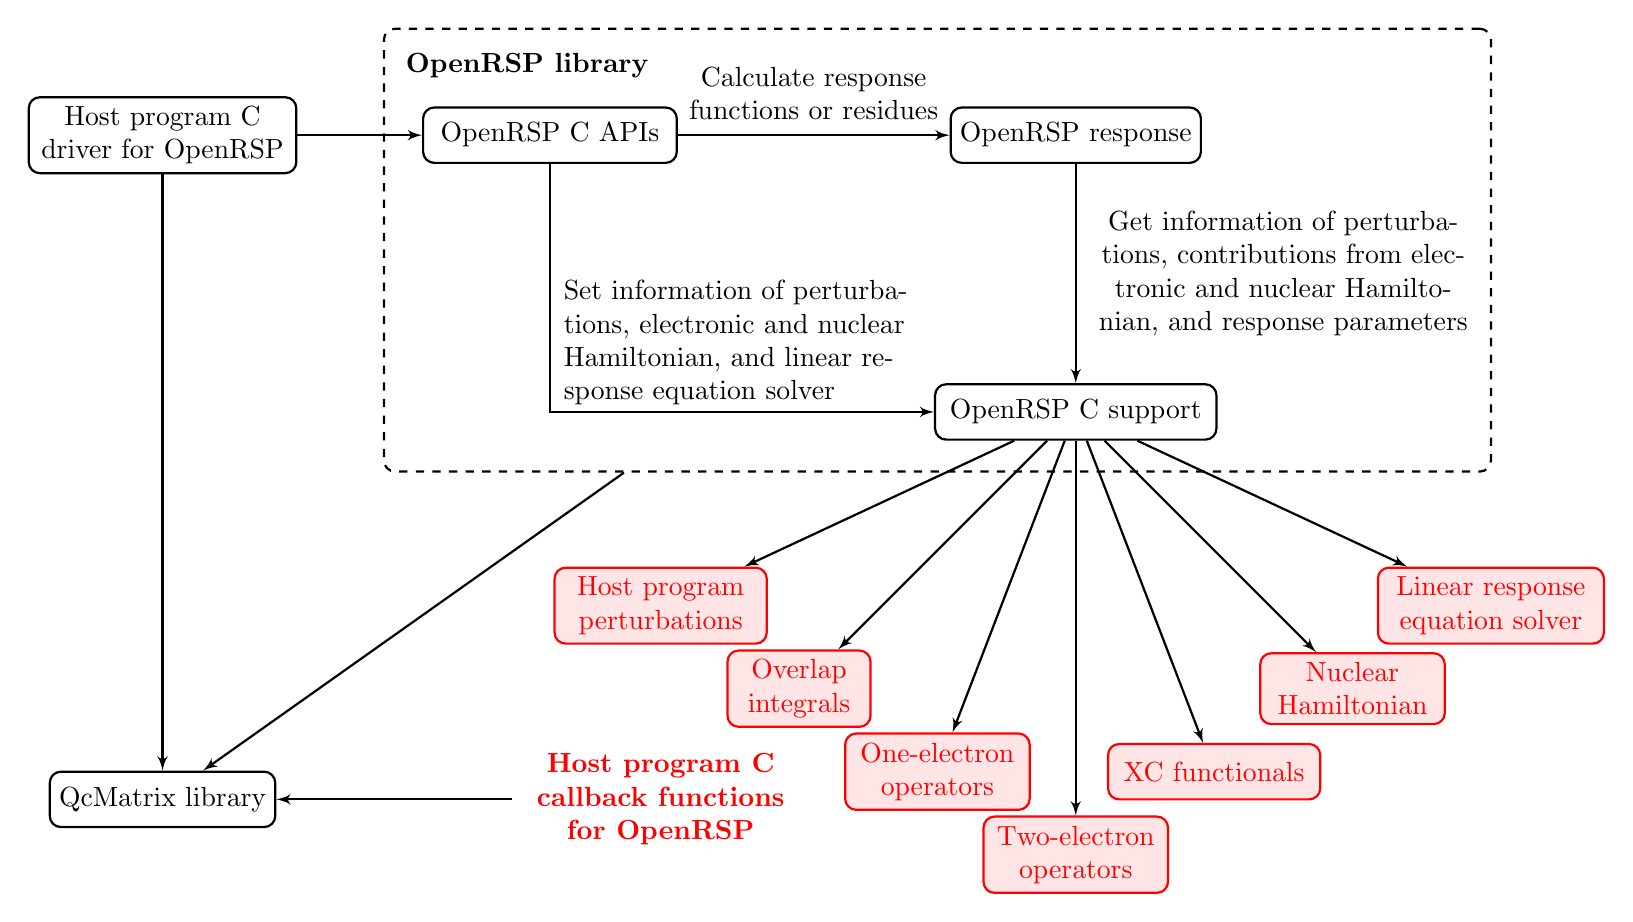
\begin{tikzpicture}[thick]
  \node[color=black, rectangle, draw, text badly centered, rounded corners, %
        minimum height=20] (OpenRSP-response) {OpenRSP response};
  \node[color=black, rectangle, draw, text badly centered, rounded corners, %
        minimum height=20, text width=85, left of=OpenRSP-response, node distance=190] %
       (OpenRSP-C-API) {OpenRSP C APIs};
  \node[color=black, rectangle, draw, text badly centered, rounded corners, %
        minimum height=20, text width=95, below of=OpenRSP-response, node distance=100] %
       (OpenRSP-C-support) {OpenRSP C support};
  \node[color=black, dashed, rectangle, draw, text badly centered, rounded corners, %
        minimum height=160, minimum width=400, above of=OpenRSP-C-API, %
        xshift=140, yshift=-70] (OpenRSP-library) %
       {\begin{minipage}[t][5cm]{13.5cm}\textbf{OpenRSP library}\end{minipage}};
%
  \node[color=black, rectangle, draw, text badly centered, rounded corners, %
        minimum height=20, text width=90, left of=OpenRSP-C-API, node distance=140] %
       (HostDriver) {Host program C driver for OpenRSP};
%
  \node[color=red, fill=red!10, rectangle, draw, text badly centered, rounded corners, %
        minimum height=20, text width=70, below of=OpenRSP-C-support, node distance=70, %
        xshift=-150, yshift=0] (Perturbations) {Host program perturbations};
  \node[color=red, fill=red!10, rectangle, draw, text badly centered, rounded corners, %
        minimum height=20, text width=45, below of=OpenRSP-C-support, node distance=70, %
        xshift=-100, yshift=-30] (Overlap) {Overlap integrals};
  \node[color=red, fill=red!10, rectangle, draw, text badly centered, rounded corners, %
        minimum height=20, text width=60, below of=OpenRSP-C-support, node distance=70, %
        xshift=-50, yshift=-60] (OneOper) {One-electron operators};
  \node[color=red, fill=red!10, rectangle, draw, text badly centered, rounded corners, %
        minimum height=20, text width=60, below of=OpenRSP-C-support, node distance=70, %
        xshift=0, yshift=-90] (TwoOper) {Two-electron operators};
  \node[color=red, fill=red!10, rectangle, draw, text badly centered, rounded corners, %
        minimum height=20, text width=70, below of=OpenRSP-C-support, node distance=70, %
        xshift=50, yshift=-60] (XCFun) {XC functionals};
  \node[color=red, fill=red!10, rectangle, draw, text badly centered, rounded corners, %
        minimum height=20, text width=60, below of=OpenRSP-C-support, node distance=70, %
        xshift=100, yshift=-30] (NucHamiltonian) {Nuclear Hamiltonian};
  \node[color=red, fill=red!10, rectangle, draw, text badly centered, rounded corners, %
        minimum height=20, text width=75, below of=OpenRSP-C-support, node distance=70, %
        xshift=150, yshift=0] (Solver) {Linear response equation solver};
  \node[color=red, text badly centered, minimum height=20, text width=100, %
        below of=HostDriver, node distance=240, xshift=180, yshift=0] (Callback) %
       {\textbf{Host program C callback functions for OpenRSP}};
%
  \node[color=black, rectangle, draw, text badly centered, rounded corners, %
        minimum height=20, below of=HostDriver, node distance=240] %
       (QcMatrix) {QcMatrix library};
%
%  \draw [-latex'] (HostDriver) edge node[align=center, midway, yshift=15, text width=120] %
%    {OpenRSP APIs (C or Fortran)} (OpenRSP);
  \draw [-latex'] (OpenRSP-C-API) edge node[align=center, midway, yshift=15, text width=120] %
    {Calculate response functions or residues} (OpenRSP-response);
  \draw [-latex'] (OpenRSP-response) edge node[align=center, midway, xshift=75, text width=160] %
    {Get information of perturbations, contributions from electronic and nuclear Hamiltonian, %
     and response parameters} (OpenRSP-C-support);
  \draw [-latex'] (OpenRSP-C-API) -- %
    node[at end, align=left, xshift=75, yshift=25, text width=140] %
    {Set information of perturbations, electronic and nuclear Hamiltonian, and linear response %
     equation solver} (OpenRSP-C-API |- OpenRSP-C-support) |- (OpenRSP-C-support);
  \draw [-latex'] (OpenRSP-library)--(QcMatrix);
  \draw [-latex'] (HostDriver)--(OpenRSP-C-API);
  \draw [-latex'] (OpenRSP-C-support)--(Perturbations);
  \draw [-latex'] (OpenRSP-C-support)--(Overlap);
  \draw [-latex'] (OpenRSP-C-support)--(OneOper);
  \draw [-latex'] (OpenRSP-C-support)--(TwoOper);
  \draw [-latex'] (OpenRSP-C-support)--(XCFun);
  \draw [-latex'] (OpenRSP-C-support)--(NucHamiltonian);
  \draw [-latex'] (OpenRSP-C-support)--(Solver);
  \draw [-latex'] (HostDriver)--(QcMatrix);
  \draw [-latex'] (Callback)--(QcMatrix);
\end{tikzpicture}

\end{document}
